
% !TeX spellcheck = en

\chapter{Flyway vs. Liquibase}

In this section, we aim to compare Flyway and Liquibase according to sources \cite{Parsick2018}, \cite{Kaps2016}, \cite{LiquibaseVSFlyway}, \cite{Zylinski2022} and our personal experience gained during this seminar.

\section{Comparison}
\marginpar{Commonalities}%
First of all, both tools use a migration-based approach for changes and are open source (Apache v2  \footnote{\url{https://github.com/flyway/flyway/blob/main/LICENSE.txt}} \footnote{\url{https://github.com/liquibase/liquibase/blob/master/LICENSE.txt}}) and in our opinion very easy to use and light-weighted.
Both offer repeatable migrations, checksum validation, and placeholder replacement and are cluster-safe.
In addition, both tools provide standard interfaces such as CLI, Java API, Maven, Ant and Spring.
The list of supported databases is almost the same for both systems, with only minor variations in supported versions or drivers. In general, there are no significant differences in terms of database support between the two systems.

\marginpar{Popularity}%
\textbf{Community}\\
Both have a similarly large community according to the references GitHub stars (Flyway: 6900, Liquibase: 3600) or tags on Stack overflow (Flyway: 2118, Liquibase 3530).

The search queries on Google also show that both receive a similar number of requests, but Liquibase is slightly ahead. The increase in searches in December 2021 is due to improvements in data collection. 
\begin{figure}[H]
	\centering
	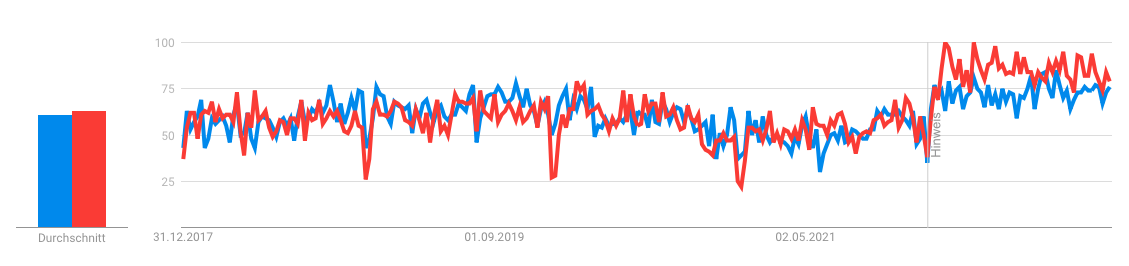
\includegraphics[width=0.9\textwidth]{./chapters/flyway_vs_liquibase/images/flyway_liquibase_search_history}
	\caption[Google Search interest over time - Source: Google Trends]{Google Search interest over time - Source: \url{trends.google.com}}
	% \label{fig:bsp_chapter:example_figure}
\end{figure}


\textbf{Integration into Existing Projects}\\
In order to be able to integrate existing projects with Flyway, one has to create a manual dump (DDL) of the production database as version 1 script, first clean and empty all other databases and migrate to version 1. Alternatively, one can manually bring the other databases to the state of the production database and set the state as version 1 using the baseline command.

On the other hand, Liquibase works the following. To tag the state of the production database as version 1, use the \package{generateChangelog} command. To compare the production database with other environments, use the diff command and generate changelogs for any differences. 
The generated changelog can be marked as "already run " or excluded from future runs.

Liquibase integration is highly promising due to the clever combination of its powerful functions. The integration of Flyway seems more like a workaround solution.

\textbf{Functionalities}\\
In the Table \ref{tab:functionalities_flyway_liquibase} you can see that Liquibase has more functionalities in the ratio 16/9. 



\begin{table}[H]
	\centering
	\ra{1.2}
	\begin{tabularx}{10cm}{X c c}
		\toprule
		Function  & 	Flyway & Liquibase \\
		\midrule
		Migration & +++ & +++ \\
		& \package{migrate} & \package{update} \\ \hline
		
		Rollback & - & ++ \\
		& \package{undo} (pro version) & \package{rollback} \\ \hline
		
		Clear schema & + & + \\
		& \package{clean} & \package{dropAll} \\ \hline
		
		Documentation & + & ++ \\
		& \package{info} & \package{DBDoc} \\ \hline
		
		Comparison & - & ++ \\
		&  & \package{Diff} \\ \hline
		
		Validation & + & - \\
		& \package{validate} & \\ \hline
		
		Initialization & + & - \\
		& \package{baseline} & \\ \hline
		
		Maintenance & + & + \\
		& \package{repair} & \package{clearChecksums} \\ \hline
		
		Callbacks & + & -\\
		& & \\ \hline
		
		Preconditions & - & + \\
		& & \\ \hline
		
		Context & - & ++ \\ 
		& & \\ \hline
		
		Refactoring & - & ++ \\
		& & \\
		\bottomrule
	\end{tabularx}
	\caption{Functionalities Flyway vs. Liquibase - Based on \cite{Zylinski2022}}
	\label{tab:functionalities_flyway_liquibase}
\end{table}





\begin{table}[H]
	\centering
		    \begin{tabular}{|l|p{.45\textwidth}|p{.45\textwidth}|}
		    \hline
			 & Liquibase & Flyway\\ \hline
			 \begin{turn}{-90}Advantages\end{turn} &
			\begin{itemize}
				\item More functionalities such as diff generation (compare two databases), Rollbacks, or monitoring and dashbording possibilities
				\item Apply the same scripts to different database vendors
				\item Integration of existing databases is more promising
				\item Work with NoSQL and relational database types
				\item DDL abstraction DSL (todo: ?)
				\item More flexible when it comes to deployment (selective deployments and rollbacks)
			\end{itemize} & \begin{itemize}
				\item Very easy and intuitive to use
				\item Direct use of SQL files
				\item Multiple schema support
				\item Clean existing schema
			\end{itemize}\\ \hline
		
	 \begin{turn}{-90}Disadvantages\end{turn} &
		\begin{itemize}
			\item Steeper learning curve and more complicated 
			\item No direct support for Java migrations
		\end{itemize} & \begin{itemize}
			\item Important features like Undo or Dry-Run are not included in the free version 
			\item No support for older Java version such as Java 6 \& 7 (enterprise only)
			\item Versioning system with linear naming convention makes it hard to manage the order of changes
		\end{itemize}\\ \hline
		\end{tabular}
	\caption{Flyway vs Liquibase comparison - Based on \cite{Parsick2018, Kaps2016}}
	\label{tab:flyway_liquivase_conparison}
\end{table}

\newpage
\section{When to use which?}

\marginpar{Question for Selection\\ \cite{Zylinski2022}, \cite{LiquibaseVSFlyway}}%
Even though both provide the essential change management functions perfectly,
their use has specific differences. With the following questions, the selection can be summed up:

\textit{Does the project use a specific database that only one tool supports?}\\
Initially, the framework conditions should be checked to determine whether a specific tool can be used. For example, Flyway cannot handle NoSQL databases, while Liquibase can. 

\textit{Do you want to continue using your previous SQL scripts 1:1?}\\
With Flyway, SQL scripts can be integrated directly. Only the name of the script would have to be adapted. When using Liquibase, the changelog files would have to be rewritten again.

\textit{Is it possible to do without rollbacks? (e.g. through clever forward migrations)}\\
Since Flyway does not offer rollbacks in the free version, the choice would fall on Liquibase. However, if one can work around this, there is no disadvantage to using Flyway.

\textit{Do you need German support?}\\
Since Liquibase is an American company, it provides information in English only. However, Flyway offers support in several languages and also in German.

\textit{Do you want to support diverse DBMS?}\\
Liquibase allows XML, YAML, or JSON to define database changes. It provides an abstraction layer better suited for software products installed in different environments with underlying database technologies. With Flyway, one writes the migrations directly in the SQL language of the used database. Therefore with Flyway, all scripts have to be rewritten for different databases. A lot can be taken over, but there is no guarantee what ends in an additional manual effort.

\textit{Are there many different environments with different database schema requirements?}\\
Liquibase is the tool of choice if this is a requirement because one can selectively deploy changes as needed to different environments. 
Liquibase supports updating and managing the same schema across multiple database vendors \& platforms using the same changelog file.
In addition, there is support to easily add new changes and reorder them without running into filename conflicts.


\newpage